\documentclass[tikz,border=3pt]{standalone}
\usepackage[T1]{fontenc}
\usepackage{lmodern,pgfplots}
\pgfplotsset{compat=1.18}
\definecolor{gapblue}{HTML}{4477AA}
\definecolor{densered}{HTML}{EE7733}
\definecolor{directgreen}{HTML}{228833}
\definecolor{inkgray}{HTML}{343A40}
\definecolor{gridgray}{HTML}{DEE3E8}
\definecolor{pendinggray}{HTML}{AAB4BE}
\newcommand{\AllianceBadge}{\tikz[baseline=-.4ex,x=.65ex,y=.65ex]{\path[fill=gapblue] (-.7,.9)--(.7,.9)--(.7,-.2)--(0,-.9)--(-.7,-.2)--cycle;}}
\newcommand{\HordeBadge}{\tikz[baseline=-.4ex,x=.65ex,y=.65ex]{\path[fill=densered] (0,1)--(.75,0)--(.45,-.8)--(0,-.45)--(-.45,-.8)--(-.75,0)--cycle;}}
\begin{document}

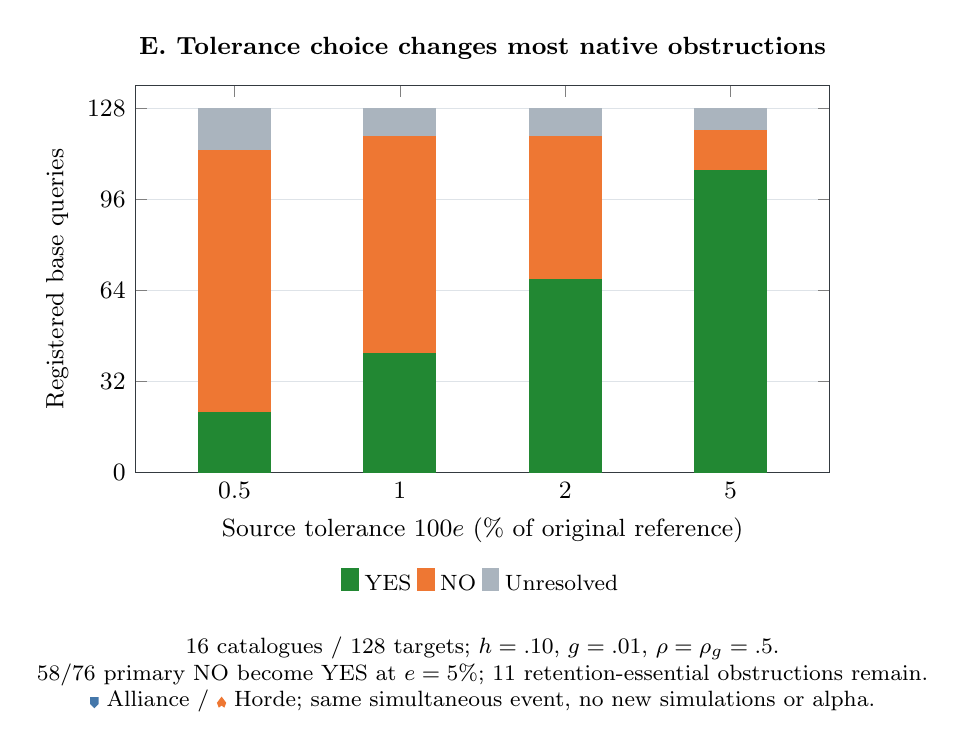
\begin{tikzpicture}
\begin{axis}[width=10.4cm,height=6.5cm,font=\small,ybar stacked,bar width=26pt,
title={E. Tolerance choice changes most native obstructions},title style={font=\small\bfseries},
xtick={0,1,2,3},xticklabels={0.5,1,2,5},xmin=-.6,xmax=3.6,
xlabel={Source tolerance $100e$ (\% of original reference)},ylabel={Registered base queries},
ymin=0,ymax=136,ytick={0,32,64,96,128},ymajorgrids,grid style={gridgray},
axis line style={inkgray},clip=false,legend style={at={(.5,-.23)},anchor=north,draw=none,legend columns=3,font=\footnotesize}]
\addplot[fill=directgreen,draw=directgreen] coordinates {(0,21) (1,42) (2,68) (3,106)};
\addlegendentry{YES}
\addplot[fill=densered,draw=densered] coordinates {(0,92) (1,76) (2,50) (3,14)};
\addlegendentry{NO}
\addplot[fill=pendinggray,draw=pendinggray] coordinates {(0,15) (1,10) (2,10) (3,8)};
\addlegendentry{Unresolved}
\node[anchor=north,align=center,font=\footnotesize] at (axis description cs:.5,-.4)
{16 catalogues / 128 targets; $h=.10$, $g=.01$, $\rho=\rho_g=.5$.\\
58/76 primary NO become YES at $e=5\%$; 11 retention-essential obstructions remain.\\
\AllianceBadge\ Alliance / \HordeBadge\ Horde; same simultaneous event, no new simulations or alpha.};
\end{axis}
\end{tikzpicture}
\end{document}
